\subsection{Hyperplane}
\begin{frame}{Maximal Margin Classifier}{Hyperplane}

    \begin{itemize}
        \item In a $p$-dimensional space, a hyperplane is a flat affine subspace of hyperplane dimension $p - 1$. It's defined as, \pause 

        \begin{equation} \label{eq:p-hyperplane}
            \beta_0 + \beta_1 X_1 + \beta_2 X_2 + \cdots + \beta_p X_p= 0
        \end{equation} \pause 

        \item We can think of the hyperplane as dividing p-dimensional space into two halves: \pause 

        \begin{align}
            \beta_0 + \beta_1 X_1 + \beta_2 X_2 + \cdots + \beta_p X_p &> 0 \\ \beta_0 + \beta_1 X_1 + \beta_2 X_2 + \cdots + \beta_p X_p &< 0
        \end{align} \pause 

        One can determine on which side of the hyperplane a point lies by simply calculating the sign of the left hand side of (\ref{eq:p-hyperplane}).
            
    \end{itemize}
\end{frame}

\subsection{Classification Using a Separating Hyperplane}
\begin{frame}{Maximal Margin Classifier}{Classification Using a Separating Hyperplane}

\begin{itemize}
    \item Supposse that we have a $n \times p$ data matrix $\textbf{X}$ that consists of $n$ training observations in $p$-dimensional space, \pause 

    \begin{equation}
    x_n = 
    \begin{pmatrix}
    x_{n1} \\
    \hdots  \\
    x_{np} 
    \end{pmatrix}.
    \end{equation} \pause 

    \item These observations fall into two classes: $y_n \in \{ -1,1 \}$ \pause 

    \item The goal is to develop a classifier based on $x_n$ that will set the test data $x^*$ into one category. \pause 

    \item Suppose that it is possible to construct a hyperplane such that, \pause 

    \begin{align}
            \beta_0 + \beta_1 x_{i1} +  \cdots + \beta_{p} X_{ip} &> 0 \text{ if } y_1 = 1 \\ 
            \beta_0 + \beta_1 x_{i1} +  \cdots + \beta_{p} X_{ip} &< 0 \text{ if } y_1 = -1
    \end{align} \pause

\end{itemize}
    
\end{frame}

\begin{frame}{Maximal Margin Classifier}{Classification Using a Separating Hyperplane}
\begin{itemize}
        \item Suppose that it is possible to construct a hyperplane such that, \pause 

    \begin{align*}
            \beta_0 + \beta_1 x_{i1} +  \cdots + \beta_{p} X_{ip} &> 0 \text{ if } y_i = 1 \\ 
            \beta_0 + \beta_1 x_{i1} +  \cdots + \beta_{p} X_{ip} &< 0 \text{ if } y_i = -1
    \end{align*} \pause
        \end{itemize}


    \begin{columns}[T]
    \column{0.4\linewidth}

        \begin{figure}
        \centering
        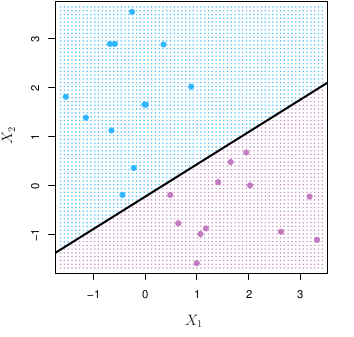
\includegraphics[height=4cm]{mmc/hyperplane.png} \pause 
    \end{figure} 

    \column{0.6\linewidth}

    \begin{itemize}
        \item If $f(x^\ast) > 0$, then $y^\ast \in 1$ \pause  
        \item If $f(x^\ast) < 0$, then $y^\ast \in -1$ \pause  
        \item If $ \mid f(x^{\ast}) \mid $ is far from zero, then this means that $x^\ast$ lies far from the hyperplane. \pause 
        \item If $ \mid f(x^{\ast}) \mid $ is close to zero, then $x^\ast$ is located near the hyperplane.
    \end{itemize}
        
    \end{columns}


    
\end{frame}

\subsection{The Maximal Margin Classifier}
\begin{frame}{Maximal Margin Classifier}{The Maximal Margin Classifier}

    \begin{itemize}
        \item In general, if our data can be perfectly separated using a hyperplane, then there will in fact exist an infinite number of such hyperplanes. \pause 

        \item Which to choose? \pause 

        \item A natural choice is the \textbf{maximal margin hyperplane (MMH)}. \pause 
        
        \item MMH is the farthest hyperplane from the training observations. \pause  

        \item To compute the farthest hyperplane, we follow the next steps: \pause 

        \begin{itemize}
            \item Compute the perpendicular distance from each training observation to a given separating hyperplane. \pause 

            \item We identify the \textbf{margin} as the smallest distance from step 1.   \pause 

            \item We identify the \textbf{MMH} as the hyperplane that correspond to the largest margin. \pause 
        \end{itemize}

        \item Then we classify a test observation based on which side of the maximal margin hyperplane it lies.
    \end{itemize}
\end{frame}

\begin{frame}{Maximal Margin Classifier}{The Maximal Margin Classifier}

\begin{figure}
    \centering
    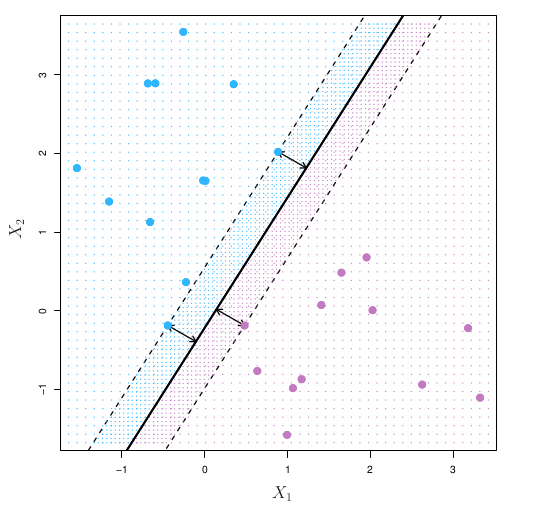
\includegraphics[height=4cm]{mmc/maximal-margin-hyperplane.png}
\end{figure}

\begin{itemize}
    \item There are 3 equidistant observations from the MMH and lie along the dashed lines indicating the width of the margin.  \pause 
    \item These are known as \textbf{support vectors}.   \pause 
    \item They “support” the MMH: if they were moved slightly then the maximal margin hyperplane would move as well.
\end{itemize}
    
\end{frame}

\subsection{Construction of the Maximal Margin Classifier}
\begin{frame}{Maximal Margin Classifier}{Construction of the Maximal Margin Classifier}

\begin{itemize}
    \item Given $n$ training observations $x_1, \cdots , x_n \in \mathbb{R}^p$ and classes $y_1, \cdots y_n \in \{ -1,1 \}$ \pause 

    \item The maximal margin hyperplane
is the solution to, \pause 

    \begin{align}
        & \max_{\beta_0, \cdots, \beta_p, M} M  \label{eq:maximize} \\
        & \text{subject to } \sum_{j=1}^p \beta_j^2 = 1, \label{eq:restriction} \\ 
        & y_i (\beta_0 + \beta_1 x_{i1} +\cdots + \beta_{p} x_{ip} )  \geq M \, \, \forall \, i = 1, \cdots, n. \label{eq:max-hyperplane}
    \end{align}\pause 

    \item Eq. (\ref{eq:max-hyperplane}) ensures that each observation will be on the correct side of the hyperplane, provided that $M$ is positive. \pause

    \item The l.h.s. of equation (\ref{eq:max-hyperplane}) is the distance from the $i$th observation to the hyperplane. \pause 

    \item So, eq. (\ref{eq:max-hyperplane}) ensures that each observation is at least a distance $M$ from the hyperplane.

\end{itemize}

    
\end{frame}

\subsection{The Non-separable Case}
\begin{frame}{Maximal Margin Classifier}{The Non-separable Case}    

\begin{itemize}
    \item The maximal margin classifier is a very natural way to perform classification, if a separating hyperplane exists. \pause 
    
    \item However, in many cases no separating hyperplane exists. \pause

    \item As we will see in the next section, we can extend the concept of a separating hyperplane in order to develop a hyperplane that almost separates the classes, using a so-called \textbf{soft margin}. \pause 

    \item The generalization of the maximal margin classifier to the
non-separable case is known as the \textbf{support vector classifier}.
\end{itemize}

\end{frame}






